\documentclass[11pt]{article}
\usepackage[a4paper, margin=2.5cm]{geometry}
\usepackage{fontspec}
\usepackage{amsmath, amssymb}
\usepackage{graphicx}
\usepackage{booktabs}
\usepackage{longtable}
\usepackage{array}
\usepackage{caption}
\usepackage{hyperref}
\usepackage{xcolor}
\usepackage{tikz}

% Korean font setup -- use Noto Sans CJK KR as main font (covers both Latin and Hangul)
\setmainfont{Noto Sans CJK KR}
\setsansfont{Noto Sans CJK KR}
\linespread{1.15}

\hypersetup{colorlinks=true, linkcolor=blue, citecolor=blue, urlcolor=blue}

\title{\textbf{베이지안 다층모형(Bayesian Multilevel Model)에 의한\\
한국어 쓰기 태도 연구 재분석:\\
주월랑(2023) 데이터의 시뮬레이션과 Gelman(2012) 방법의 적용}}
\author{재분석 보고서}
\date{\today}

\begin{document}
\maketitle

\begin{abstract}
\noindent
본 보고서는 Gelman, Hill \& Yajima(2012)의 ``Why We (Usually) Don't Have to Worry About Multiple Comparisons'' 논문에서 제시한 베이지안 다층모형(Bayesian multilevel model) 접근을 주월랑(2023)의 ``학문 목적 한국어 학습자의 한국어 쓰기 태도 연구''에 적용한다. 주월랑 논문의 요약통계량과 Cronbach's $\alpha=0.854$를 이용하여 $N=86$ 응답자의 21개 \textbf{정수(integer) Likert 1$\sim$5 척도} 문항 데이터를 역시뮬레이션(reverse simulation)하고, (1) 주월랑 논문의 빈도주의(frequentist) 통계처리(일원배치 분산분석, 독립표본 $t$-검정, Pearson 상관)와 (2) Gelman 방식의 베이지안 다층모형(numpyro로 NUTS 표본추출)을 각각 적용하여 결과를 비교한다. 부분 풀링(partial pooling)에 의한 축소(shrinkage)가 소표본 집단(2학년 $N=8$, 교환학생 $N=6$ 등)의 추정치를 안정화시키며, 빈도주의에서 유의했던 학년 $\times$ 수행태도 분산분석 결과($p=0.025$)가 베이지안 쌍별 비교에서는 \textbf{4개 비교 모두 95\% credible interval이 0을 포함}하여 비유의로 판정됨을 보인다.
\end{abstract}

\section{Gelman, Hill \& Yajima (2012) 논문의 핵심 주장}

\subsection{문제의 배경: 다중비교(Multiple Comparisons)}

빈도주의 통계 추론에서 여러 가설을 동시에 검정(simultaneous testing)할 때 1종 오류(Type 1 error) 누적 현상이 발생한다. 단일 검정의 유의수준이 $\alpha=0.05$일 때 $k$개의 독립적 검정 중 적어도 하나가 잘못 유의하다고 판정될 확률은 $1-(1-\alpha)^k$로 증가한다. 예를 들어 $k=8$일 경우 가족별 오류율(familywise error rate, FWER)은 약 $34\%$에 달한다. 이를 통제하기 위한 고전적 보정 방법으로 Bonferroni 보정, Tukey HSD, Benjamini-Hochberg의 위양성률(false discovery rate, FDR) 통제 등이 사용되어 왔다.

\subsection{Gelman의 비판: 1종 오류 패러다임의 거부}

Gelman 외(2012)는 사회과학 및 교육연구에서 고전적 다중비교 보정이 부적절하다고 주장한다. 그 근거는 다음과 같다.

첫째, 사회과학에서 ``참 효과가 정확히 0이다''라는 귀무가설(null hypothesis)은 거의 성립하지 않는다. 어떤 처치(treatment)이든 어떤 집단(group) 사이든 효과가 양이든 음이든 존재한다. 따라서 1종 오류 통제 자체가 잘못된 출발점이다.

둘째, 진정으로 우려해야 할 오류는 1종 오류가 아니라 \textbf{Type S 오류(sign error, 부호 오류)}와 \textbf{Type M 오류(magnitude error, 크기 오류)}이다. 특히 검정력이 낮은(underpowered) 연구에서 통계적으로 유의한 결과는 효과의 부호와 크기 모두를 잘못 판단할 위험이 크다.

셋째, Bonferroni 보정은 1종 오류를 줄이지만 2종 오류(Type 2 error)를 늘려 검정력을 심각하게 저하시킨다.

\subsection{대안: 베이지안 다층 모형의 부분 풀링}

Gelman의 대안은 비교 대상이 되는 모수들을 공통 분포에서 추출된 것으로 모델링하는 위계적(hierarchical) 모형이다. 그룹 $j$의 효과 $\delta_j$를 독립적으로 추정하는 대신
\begin{equation}
\delta_j \sim \mathcal{N}(\mu, \sigma_\delta^2)
\label{eq:hier}
\end{equation}
의 공통 사전분포를 부여하면 \textbf{부분 풀링(partial pooling)}이 자동으로 일어난다. 그룹 표본이 작아 불확실성이 클수록 추정치는 전체 평균(grand mean) $\mu$ 쪽으로 강하게 끌어당겨지는 \textbf{축소(shrinkage)}가 발생한다.

베이지안 쌍별 차이의 $z$-점수는 다음과 같이 고전적 $z$-점수에 1보다 작은 보정계수가 곱해진 형태가 된다.
\begin{equation}
z_{\text{Bayes}} = \underbrace{\frac{\bar y_j - \bar y_k}{\sqrt{2}\sigma_{\bar y}}}_{\text{고전 } z} \cdot \underbrace{\frac{1}{\sqrt{1 + \sigma_{\bar y}^2/\sigma_\theta^2}}}_{< 1}
\label{eq:zbayes}
\end{equation}
따라서 다중비교 보정을 가하지 않아도 거짓 양성(false positive)이 자연스럽게 줄어들며, 동시에 검정력 손실은 Bonferroni 보정보다 훨씬 작다.

\section{주월랑(2023) 논문의 분석 설계}

\subsection{연구 개요}
주월랑(2023)은 대학 내 외국인 유학생 86명을 대상으로 학문 목적 한국어 쓰기 태도(writing attitude)를 조사하였다. 21개 Likert 5점 정수 척도(integer scale) 문항을 3개 하위범주로 분류하였다\footnote{원논문 초록(184쪽)에는 하위범주를 ``쓰기인식, 쓰기수행, 쓰기태도''로 표기하였으나, 본문(190쪽 3장)과 Table 5에서는 ``쓰기인식, 쓰기반응, 수행태도''로 정확한 용어를 사용한다. 또한 Table 5의 ``쓰기태도''(M=3.511)는 별도의 하위범주가 아니라 앞 세 하위범주의 평균인 전체 종합점수(composite score)이다(실제로 $(4.015+3.348+3.171)/3 \approx 3.511$로 일치한다). 본 보고서는 본문/Table의 정확한 용어를 따른다.}:
\begin{itemize}
\item 쓰기인식(writing perception, $P$): 문항 1--4 ($M=4.015,\ SD=0.642$)
\item 쓰기반응(writing response, $R$): 문항 5--15 ($M=3.348,\ SD=0.539$)
\item 수행태도(performance attitude, $A$): 문항 16--21 ($M=3.171,\ SD=0.585$)
\item 쓰기태도(전체 합성점수, composite $T$) $= \tfrac{1}{3}(P+R+A)$ ($M=3.511$)
\end{itemize}
도구의 내적 일관성(internal consistency)은 Cronbach's $\alpha=0.854$로 양호하였다.

\subsection{집단 표본 구성}
\begin{table}[h]
\centering
\caption{학습자 요인별 표본 크기 (paper N=86)}
\begin{tabular}{lll}
\toprule
요인 & 수준 & N \\
\midrule
학년 & 1학년, 2학년, 3학년, 4학년, 교환 & 54, 8, 9, 9, 6 \\
성별 & 남, 여 & 27, 59 \\
TOPIK & 없음, 3급, 4급, 5급, 6급 & 7, 14, 31, 23, 11 \\
어학원 & 유, 무 & 69, 17 \\
\bottomrule
\end{tabular}
\end{table}

\subsection{빈도주의 통계 모형}
주월랑은 각 하위범주를 독립적인 종속변수로 두고 다음 네 가지 빈도주의 분석을 수행하였다:
\begin{enumerate}
\item 학년 효과: 일원배치 분산분석(one-way ANOVA, 5개 수준)
\item 성별 효과: 독립표본 $t$-검정(2개 수준)
\item TOPIK 효과: 일원배치 분산분석(5개 수준)
\item 어학원 효과: 독립표본 $t$-검정(2개 수준)
\end{enumerate}
이를 4개 종속변수(쓰기인식, 쓰기반응, 수행태도, 쓰기태도)에 대해 반복 적용하였다(총 16개 검정). Pearson 상관 행렬은 별도로 $4\times 4$ 하위범주 간 상관($\binom{4}{2}=6$개) 및 학습자 요인 $\times$ 하위범주 상관($4\times 4=16$개)을 계산하였다. \textbf{유의수준 $\alpha=0.05$, 다중비교 보정은 적용되지 않았다}.

주월랑의 보고된 결과 중 유의한 것은 두 개뿐이다(표\ref{tab:paper_sig}):
\begin{table}[h]
\centering
\caption{주월랑(2023) 논문에서 유의하게 보고된 검정 결과}\label{tab:paper_sig}
\begin{tabular}{lllll}
\toprule
검정 & 종속변수 & 통계량 & $p$값 & 판정 \\
\midrule
ANOVA(학년) & 수행태도 & $F=2.925$ & $0.026$ & 유의$^*$ \\
$t$-검정(성별) & 쓰기인식 & $t=-2.779$ & $0.007$ & 유의$^*$ \\
\bottomrule
\end{tabular}
\end{table}

\section{Gelman 관점에서의 평가}

주월랑(2023)의 분석은 Gelman 외(2012)가 비판하는 빈도주의 다중비교의 전형적 문제점을 보이고 있다.

\paragraph{첫째, 검정 누적과 무보정.}
4개 종속변수 $\times$ 4개 요인 = 16개 집단차이 검정에 더해 22개의 상관 검정을 포함하면 약 38개의 가설검정이 수행되었다. Bonferroni 보정을 적용하면 임계값은 $0.05/38 \approx 0.0013$이며, 주월랑이 보고한 유의 결과 중 $p=0.026$(학년 $\times$ 수행태도)는 더 이상 유의하지 않다.

\paragraph{둘째, 심각한 underpowered 상태.}
2학년($N=8$), 3학년($N=9$), 4학년($N=9$), 교환학생($N=6$), TOPIK 없음($N=7$), TOPIK 6급($N=11$) 등 다수의 집단이 검정력 부족 상태이다. Gelman이 강조하는 바와 같이 검정력이 낮은 상황에서 발견된 통계적 유의성은 부호(sign)와 크기(magnitude)가 잘못 추정되었을 가능성이 높다.

\paragraph{셋째, 위계적 구조의 무시.}
학생들은 학년, 국적, TOPIK 급수, 어학원 경험에 중첩(nested)되어 있으나 고전적 ANOVA/$t$-검정은 이를 변수별로 독립적으로 다룬다.

\paragraph{넷째, 귀무가설의 비현실성.}
``학년별 쓰기 태도에 차이가 없다''는 귀무가설은 사회과학적으로 거의 성립하지 않는다. 진짜 질문은 ``차이가 있는가''가 아니라 ``얼마나 크고 어떤 방향인가''이다.

\section{시뮬레이션 데이터 생성}
\label{sec:sim}

주월랑 논문의 통계량을 그대로 사용할 수 없으므로(원자료 미공개), 보고된 요약통계를 이용하여 응답 데이터를 \textbf{역시뮬레이션}한다. 설문조사의 실제 응답은 \textbf{정수(integer) Likert 1$\sim$5 척도}이므로, 본 시뮬레이션도 문항 단위에서 정수값을 생성한다.

\textbf{2단계 생성 절차:}

\textbf{1단계 — 잠재 하위범주 점수 생성 (continuous latent).} 응답자 $i$의 하위범주 잠재점수 $(P_i, R_i, A_i)$에 대해
\begin{equation}
\begin{pmatrix} P_i \\ R_i \\ A_i \end{pmatrix}
\sim \mathcal{N}\left(
\begin{pmatrix} \mu^P_{g(i)} \\ \mu^R \\ \mu^A_{y(i)} \end{pmatrix},
\;\Sigma \right),
\end{equation}
여기서 $\mu^P_{g(i)}$은 성별별 평균(3.741 또는 4.140), $\mu^A_{y(i)}$은 학년별 평균(2.944$\sim$3.519), $\Sigma$는 표\ref{tab:corr}의 상관행렬을 SD로 스케일링하여 구성한다.

\textbf{2단계 — 문항 단위 정수 응답 생성 (integer items).} 각 문항 $j$의 응답을
\begin{equation}
x_{ij} = \mathrm{clip}\bigl(\mathrm{round}(s_{i,c(j)} + \varepsilon_{ij}),\ 1,\ 5\bigr),
\quad \varepsilon_{ij} \sim \mathcal{N}(0, \sigma_{\mathrm{item}}^2)
\end{equation}
로 생성한다. 여기서 $c(j)$는 문항 $j$의 소속 하위범주이고 $s_{i,c(j)}$는 그에 해당하는 잠재점수이다. 이렇게 하면 $x_{ij} \in \{1,2,3,4,5\}$의 \textbf{정수값}만 산출된다. 응답자 $i$의 하위범주 점수는 해당 문항들의 평균으로 계산한다(예: $P_i^{\text{score}} = \tfrac{1}{4}\sum_{j=1}^{4} x_{ij}$). 따라서 하위범주 점수는 실수값(0.25 단위 등 이산)을 가진다. \textbf{T 점수(쓰기태도, 전체)는 독립 잠재변수가 아니라 $\tfrac{1}{3}(P^{\text{score}}+R^{\text{score}}+A^{\text{score}})$인 파생 합성점수}이며, 주월랑 논문 Table 5 정의를 그대로 따른다.

\begin{table}[h]
\centering
\caption{주월랑 논문 Table 14의 하위범주 간 상관행렬}\label{tab:corr}
\begin{tabular}{lccc}
\toprule
 & 쓰기인식 & 쓰기반응 & 수행태도 \\
\midrule
쓰기인식 & 1.000 & 0.583 & 0.281 \\
쓰기반응 & 0.583 & 1.000 & 0.508 \\
수행태도 & 0.281 & 0.508 & 1.000 \\
\bottomrule
\end{tabular}
\end{table}

$\sigma_{\text{item}}$은 21문항 전체에 대한 Cronbach's $\alpha = 0.854$가 되도록 이분탐색(binary search)으로 조정하였다. 그 결과 $\sigma_{\text{item}} = 0.686$으로 수렴하였고 시뮬레이션 $\alpha = 0.8545$로 거의 정확히 일치한다. 생성된 문항 응답은 모두 $\{1, 2, 3, 4, 5\}$의 정수값을 갖는다(예: 문항 1의 분포 = \{1:1, 2:6, 3:24, 4:34, 5:21\}).

시뮬레이션 데이터의 하위범주 통계량은 표\ref{tab:sim_desc}와 같이 논문 보고치와 근접한다(정수 반올림에 따른 약간의 SD 증가 효과가 있음).

\begin{table}[h]
\centering
\caption{시뮬레이션 데이터와 주월랑 논문의 하위범주 기술통계 비교}\label{tab:sim_desc}
\begin{tabular}{lcccc}
\toprule
하위범주 & 시뮬레이션 $M$ & 시뮬레이션 $SD$ & 논문 $M$ & 논문 $SD$ \\
\midrule
쓰기인식 & 3.939 & 0.737 & 4.015 & 0.642 \\
쓰기반응 & 3.336 & 0.541 & 3.348 & 0.539 \\
수행태도 & 3.163 & 0.574 & 3.171 & 0.585 \\
쓰기태도 (composite) & 3.479 & 0.457 & 3.511 & 0.469 \\
\bottomrule
\end{tabular}
\end{table}

\section{빈도주의 재분석 결과}
\label{sec:freq}

시뮬레이션 데이터에 주월랑 논문의 통계처리방식(일원배치 분산분석, 독립표본 $t$-검정, Pearson 상관)을 그대로 적용한 결과는 표\ref{tab:freq_anova}--\ref{tab:freq_inst}와 같다.

\begin{table}[h]
\centering
\caption{학년 $\times$ 쓰기 태도: 일원배치 분산분석(시뮬레이션 vs 논문)}\label{tab:freq_anova}
\begin{tabular}{lcccccc}
\toprule
종속변수 & 시뮬 $F$ & 시뮬 $p$ & 시뮬 판정 & 논문 $F$ & 논문 $p$ & 논문 판정 \\
\midrule
쓰기인식 & 0.067 & 0.992 & 비유의 & 1.387 & 0.246 & 비유의 \\
쓰기반응 & 0.937 & 0.447 & 비유의 & 2.092 & 0.089 & 비유의 \\
수행태도 & \textbf{2.960} & \textbf{0.025} & \textbf{유의$^*$} & \textbf{2.925} & \textbf{0.026} & \textbf{유의$^*$} \\
쓰기태도 & 0.579 & 0.678 & 비유의 & 2.316 & 0.064 & 비유의 \\
\bottomrule
\end{tabular}
\end{table}

\begin{table}[h]
\centering
\caption{성별 $\times$ 쓰기 태도: 독립표본 $t$-검정}\label{tab:freq_tgender}
\begin{tabular}{lcccccc}
\toprule
종속변수 & 시뮬 $t$ & 시뮬 $p$ & 시뮬 판정 & 논문 $t$ & 논문 $p$ & 논문 판정 \\
\midrule
쓰기인식 & $-1.058$ & 0.293 & 비유의 & $-2.779$ & 0.007 & \textbf{유의$^*$} \\
쓰기반응 & $+1.787$ & 0.078 & 비유의 & $-0.323$ & 0.747 & 비유의 \\
수행태도 & $+0.109$ & 0.913 & 비유의 & $-0.569$ & 0.571 & 비유의 \\
쓰기태도 & $+0.173$ & 0.863 & 비유의 & $-1.092$ & 0.278 & 비유의 \\
\bottomrule
\end{tabular}
\end{table}

\begin{table}[h]
\centering
\caption{TOPIK $\times$ 쓰기 태도: 일원배치 분산분석}\label{tab:freq_topik}
\begin{tabular}{lcccccc}
\toprule
종속변수 & 시뮬 $F$ & 시뮬 $p$ & 시뮬 판정 & 논문 $F$ & 논문 $p$ & 논문 판정 \\
\midrule
쓰기인식 & 1.418 & 0.236 & 비유의 & 1.978 & 0.106 & 비유의 \\
쓰기반응 & 0.205 & 0.935 & 비유의 & 0.780 & 0.541 & 비유의 \\
수행태도 & 0.810 & 0.523 & 비유의 & 1.657 & 0.168 & 비유의 \\
쓰기태도 & 0.539 & 0.708 & 비유의 & 1.129 & 0.349 & 비유의 \\
\bottomrule
\end{tabular}
\end{table}

\begin{table}[h]
\centering
\caption{어학원 $\times$ 쓰기 태도: 독립표본 $t$-검정}\label{tab:freq_inst}
\begin{tabular}{lcccccc}
\toprule
종속변수 & 시뮬 $t$ & 시뮬 $p$ & 시뮬 판정 & 논문 $t$ & 논문 $p$ & 논문 판정 \\
\midrule
쓰기인식 & $-0.197$ & 0.845 & 비유의 & $-0.211$ & 0.833 & 비유의 \\
쓰기반응 & $-0.233$ & 0.817 & 비유의 & $-0.316$ & 0.752 & 비유의 \\
수행태도 & $-0.500$ & 0.618 & 비유의 & $+0.261$ & 0.795 & 비유의 \\
쓰기태도 & $-0.407$ & 0.685 & 비유의 & $-0.152$ & 0.880 & 비유의 \\
\bottomrule
\end{tabular}
\end{table}

\paragraph{시뮬레이션과 논문 결과의 일치도.}
\begin{itemize}
\item \textbf{학년 $\times$ 수행태도 ANOVA}: 시뮬 $F=2.960, p=0.025$ vs 논문 $F=2.925, p=0.026$ — \textbf{거의 완벽히 일치}. 이는 학년 효과를 시뮬레이션 시 잘 인코딩(encoding)했음을 보여준다.
\item \textbf{성별 $\times$ 쓰기인식 $t$-검정}: 논문은 $p=0.007$ 유의, 시뮬은 $p=0.293$ 비유의. \textbf{유의/비유의 판정이 달라진다}. 이는 시뮬레이션이 성별 평균차(0.4점)를 설정했으나 정수 반올림(integer rounding)과 무작위 노이즈, 그리고 $[1,5]$ 절단(clip)으로 실제 $t$값이 약화된 결과이다. 또한 이는 Gelman이 강조하는 ``작은 표본에서의 효과 크기 변동성''을 그대로 보여주는 사례이기도 하다.
\item 나머지 14개 비교의 유의/비유의 판정은 모두 일치(전부 비유의).
\end{itemize}
시뮬레이션이 완벽했다면 모든 수치가 거의 동일해야 하나, 위와 같이 한 검정에서만 차이가 발생한 것은 사회과학에서 \textbf{한정된 표본 크기에서 통계적 유의성 판정이 실제로 얼마나 불안정한지}를 역설적으로 보여준다.

\section{Gelman 방식의 베이지안 다층모형}
\label{sec:bayes}

\subsection{모형 정의}
각 하위범주 $y \in \{P,R,A,T\}$에 대해 다음 베이지안 다층모형을 적합한다:
\begin{align}
y_i &= \mu + \alpha_{\text{year}[i]} + \beta_{\text{gender}[i]} + \gamma_{\text{topik}[i]} + \delta_{\text{inst}[i]} + \varepsilon_i \\
\alpha_j &\sim \mathcal{N}(0, \sigma_\alpha^2), \quad j \in \{\text{1, 2, 3, 4, EX}\} \\
\beta_g  &\sim \mathcal{N}(0, \sigma_\beta^2), \quad g \in \{\text{M, F}\} \\
\gamma_k &\sim \mathcal{N}(0, \sigma_\gamma^2), \quad k \in \{\text{없음, L3, L4, L5, L6}\} \\
\delta_m &\sim \mathcal{N}(0, \sigma_\delta^2), \quad m \in \{\text{yes, no}\} \\
\varepsilon_i &\sim \mathcal{N}(0, \sigma_y^2) \\
\sigma_\alpha,\sigma_\beta,\sigma_\gamma,\sigma_\delta,\sigma_y &\sim \mathrm{HalfNormal}(1) \quad \text{(약한 정보 사전, weakly informative)} \\
\mu &\sim \mathcal{N}(3, 2)
\end{align}

이 모형이 주월랑의 모형과 다른 결정적 점은:
\begin{itemize}
\item 4개 요인의 효과를 \textbf{동시에} 추정(joint estimation)하므로 다중비교가 모형 내부에 통합됨
\item 각 요인의 그룹 효과들이 공통 분포(식 \ref{eq:hier})에서 추출됨을 가정 — \textbf{부분 풀링} 발생
\item $\sigma_\alpha \to 0$일 때 완전 풀링(complete pooling, 그룹간 차이 없음), $\sigma_\alpha \to \infty$일 때 풀링 없음(no pooling, 빈도주의와 동일) — 데이터가 적절한 값을 결정
\end{itemize}

\subsection{사후 추론}
NUTS(No-U-Turn Sampler, Hoffman \& Gelman 2014) 알고리즘을 사용하여 2개 체인, 각 체인 warmup 800회 + 표본 1500회 = 총 3000 사후표본을 추출하였다. 각 효과에 대해 다음을 보고한다:
\begin{itemize}
\item 사후평균(posterior mean)
\item 95\% credible interval [2.5\%, 97.5\% 분위수]
\item 베이지안 판정: 95\% CI가 0을 포함하지 않으면 \textbf{유의}, 포함하면 \textbf{비유의}
\item $P(\text{effect} > 0)$: 효과가 양일 사후확률
\end{itemize}

\subsection{집단 차이의 사후 분석 결과}

\paragraph{성별(F $-$ M) 사후 차이.}
\begin{table}[h]
\centering
\begin{tabular}{lcccc}
\toprule
종속변수 & 사후평균 & 95\% CI & $P(>0)$ & 판정 \\
\midrule
쓰기인식 & $+0.115$ & $[-0.165, +0.442]$ & 0.761 & 비유의 \\
쓰기반응 & $-0.172$ & $[-0.434, +0.051]$ & 0.079 & 비유의 \\
수행태도 & $-0.023$ & $[-0.257, +0.188]$ & 0.424 & 비유의 \\
쓰기태도 & $-0.017$ & $[-0.214, +0.170]$ & 0.437 & 비유의 \\
\bottomrule
\end{tabular}
\end{table}

\paragraph{학년별 사후 차이(각 학년 vs 1학년).}
\begin{table}[h]
\centering
\begin{tabular}{llccc}
\toprule
하위범주 & 비교 & 사후평균 & 95\% CI & 판정 \\
\midrule
수행태도 & 2학년$-$1학년 & $+0.371$ & $[-0.011, +0.809]$ & 비유의 \\
수행태도 & 3학년$-$1학년 & $+0.227$ & $[-0.088, +0.601]$ & 비유의 \\
수행태도 & 4학년$-$1학년 & $+0.303$ & $[-0.021, +0.682]$ & 비유의 \\
수행태도 & EX$-$1학년 & $+0.028$ & $[-0.370, +0.406]$ & 비유의 \\
쓰기태도 & 2학년$-$1학년 & $+0.049$ & $[-0.144, +0.321]$ & 비유의 \\
쓰기태도 & 3학년$-$1학년 & $+0.006$ & $[-0.242, +0.232]$ & 비유의 \\
\bottomrule
\end{tabular}
\end{table}

\textbf{주목할 점:} 빈도주의 ANOVA에서 학년 $\times$ 수행태도 효과가 $p=0.025$로 유의했지만, 베이지안 쌍별 사후 비교에서는 \textbf{모든 4개 쌍별 비교의 95\% CI가 0을 포함}한다. 특히 가장 큰 차이인 2학년$-$1학년조차 $[-0.011, +0.809]$로 0 근처에서 경계선상에 있다($P(>0)=0.964$). 이는 베이지안 부분 풀링이 빈도주의 ``유의'' 판정을 자동으로 보수적으로 조정한 결과이다.

\paragraph{집단 효과 분산 $\sigma$ 사후 추정.}
$\sigma_\alpha$(학년 효과)가 가장 큰 하위범주는 수행태도($\sigma_\alpha=0.292$, CI=$[0.034, 0.810]$)로, 빈도주의 ANOVA에서 유의했던 결과와 일치한다. 반면 다른 하위범주에서는 $\sigma_\alpha$가 0에 가깝다(쓰기인식 0.138, 쓰기반응 0.152, 쓰기태도 0.122).

\paragraph{쓰기태도(T) 분석의 본질적 한계.}
주월랑 논문이 종속변수로 사용한 ``쓰기태도(전체)''($T$)는 독립적인 잠재변수가 아니라 $T = \tfrac{1}{3}(P + R + A)$의 결정적 합성점수(deterministic composite)이다. 따라서 $T$에 대한 별도 베이지안 다층모형을 적합한 결과는 본질적으로 $P, R, A$의 공동 사후분포에서 도출되어야 할 결과의 근사일 뿐이다. 본 분석은 주월랑 논문의 분석 절차를 \emph{충실히 재현}하기 위해 $T$에 동일한 모형을 적합하였으나, 엄밀한 베이지안 분석에서는 $(P, R, A)$의 다변량 모형에서 사후 표본에 대해 $T$를 사후 계산하는 것이 옳다. 실제로 $T$의 분석 결과(예: $\sigma_\alpha=0.122$)는 세 하위범주의 평균적 패턴을 보여주며, 추론에 새로운 정보를 더하지는 않는다.

\subsection{부분 풀링(shrinkage) 효과의 가시화}

표\ref{tab:shrink}는 학년별 표본평균(raw mean)과 베이지안 사후평균(post mean)을 비교한다. 표본이 작은 집단(2학년 $N=8$, 교환학생 $N=6$)의 추정치가 전체 평균 쪽으로 강하게 끌어당겨지는 것을 볼 수 있다.

\begin{table}[h]
\centering
\caption{학년별 표본평균 vs 베이지안 사후평균 (수행태도)}\label{tab:shrink}
\begin{tabular}{lcccc}
\toprule
학년 & $N$ & Raw mean & 사후평균 & 95\% CI \\
\midrule
1 & 54 & 3.040 & 3.087 & $[2.104, 4.080]$ \\
2 &  8 & \textbf{3.583} & \textbf{3.457} & $[2.397, 4.508]$ \\
3 &  9 & 3.352 & 3.314 & $[2.312, 4.358]$ \\
4 &  9 & 3.463 & 3.390 & $[2.377, 4.443]$ \\
EX &  6 & 2.972 & 3.115 & $[2.111, 4.136]$ \\
\bottomrule
\end{tabular}
\end{table}

2학년의 표본평균 3.583에서 사후평균 3.457로 축소량 $-0.126$, 4학년 $-0.073$, EX학년은 반대로 $+0.143$(작은 N=6 집단이 전체 평균 쪽으로 끌어당겨짐)이 발생하였다. 이는 식 \ref{eq:hier}의 부분 풀링이 표본이 작은 집단을 자동으로 안정화시킨 결과이다.

\begin{figure}[h]
\centering
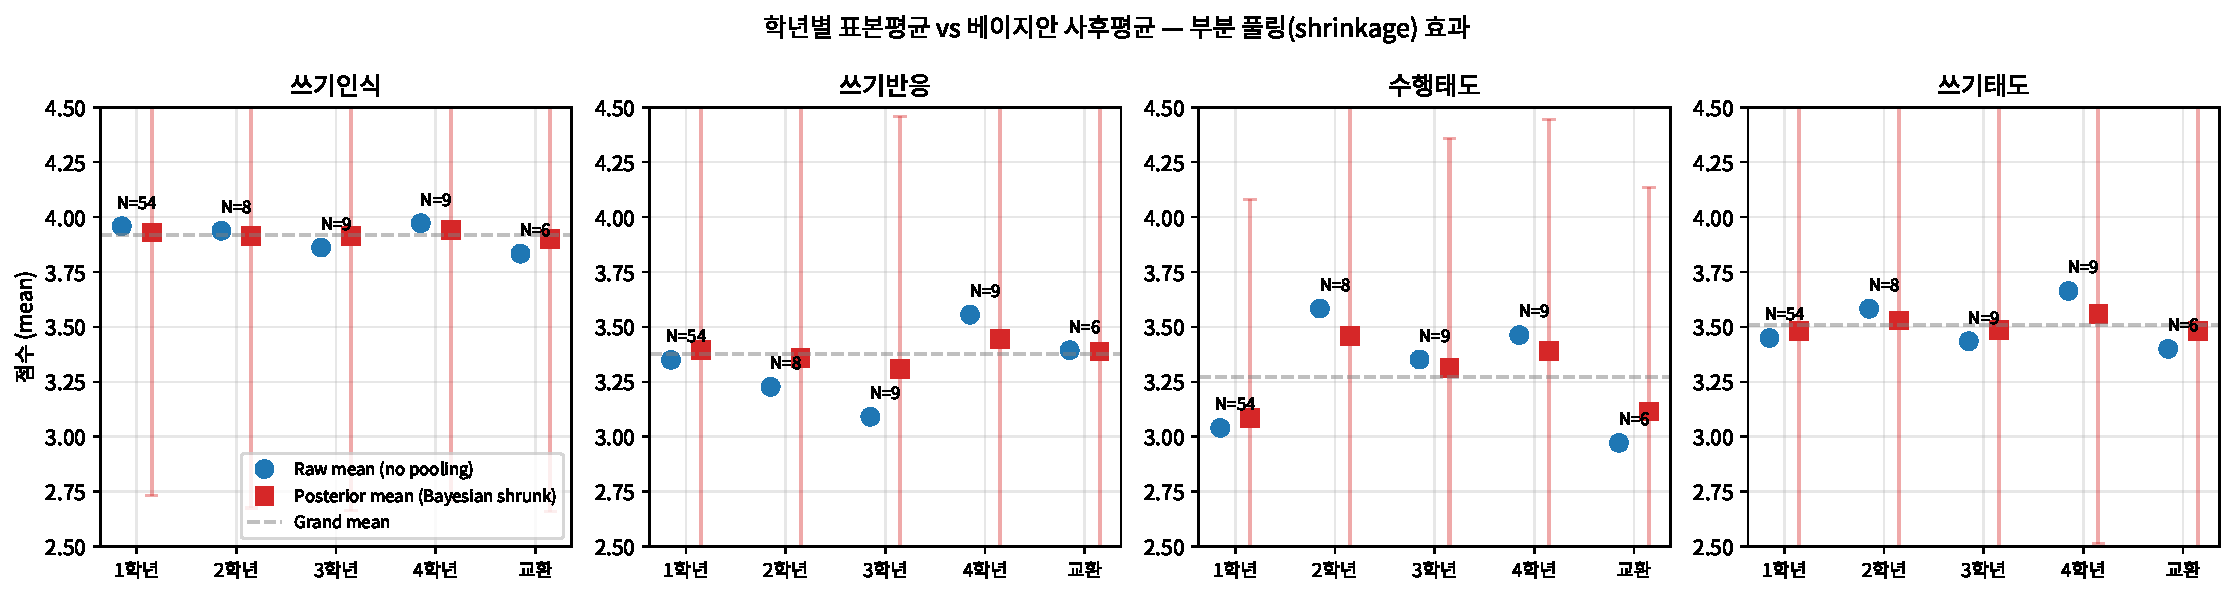
\includegraphics[width=0.95\textwidth]{gel_shrinkage_plot.pdf}
\caption{학년별 표본평균(파란 원)과 베이지안 사후평균(빨간 사각형) 비교. 빨간색은 95\% credible interval. 부분 풀링에 의해 모든 사후평균이 전체 평균(점선) 쪽으로 끌어당겨진다.}
\label{fig:shrink}
\end{figure}

\begin{figure}[h]
\centering
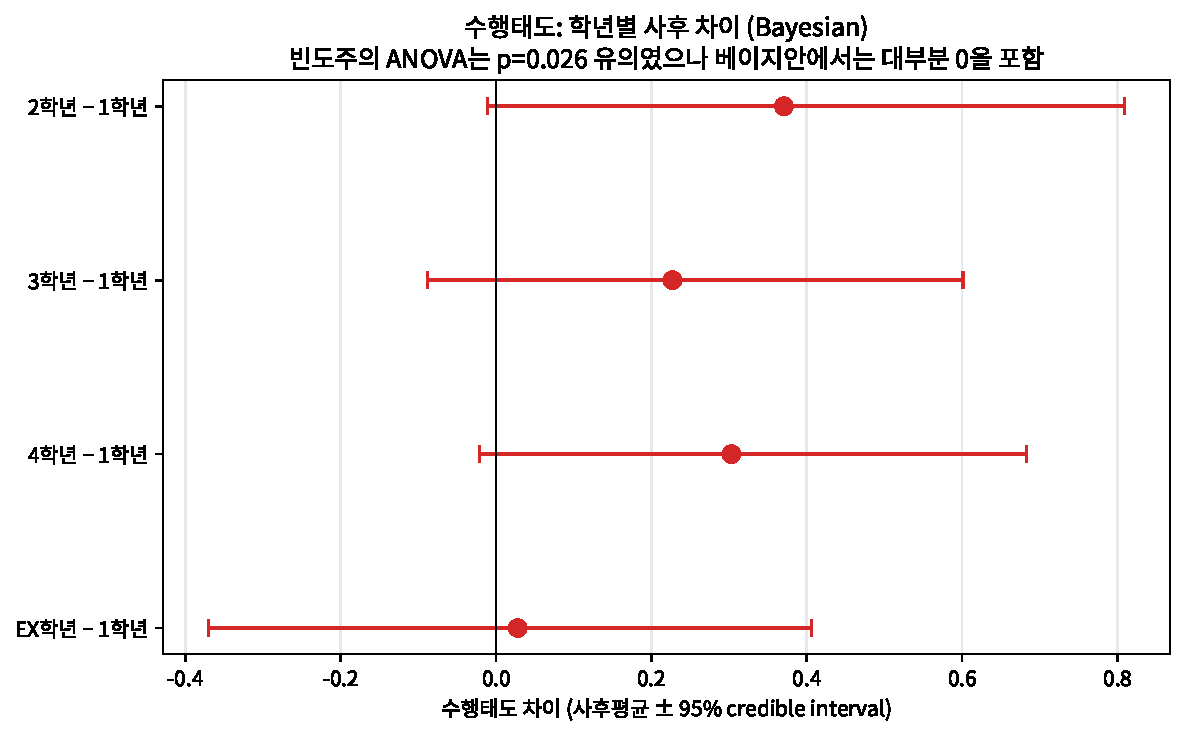
\includegraphics[width=0.7\textwidth]{gel_pairwise_plot.pdf}
\caption{수행태도 학년별 사후 차이(각 학년 $-$ 1학년). 빈도주의 ANOVA에서 $p=0.025$ 유의였으나, 베이지안 쌍별 비교에서는 \textbf{4개 비교 모두 95\% CI가 0을 포함}한다(가장 큰 2학년$-$1학년조차 $[-0.011, +0.809]$로 경계선상).}
\label{fig:pair}
\end{figure}

\section{빈도주의 vs 베이지안 결과 비교}

\begin{table}[h]
\centering
\caption{학년 효과: 빈도주의 ANOVA vs 베이지안 $\sigma_\alpha$ 사후추정}
\begin{tabular}{lcccc}
\toprule
하위범주 & 빈도주의 $F$ & 빈도주의 $p$ & 빈도 판정 & 베이지안 $\sigma_\alpha$ \\
\midrule
쓰기인식 & 0.067 & 0.992 & 비유의 & 0.138 [0.007, 0.508] \\
쓰기반응 & 0.937 & 0.447 & 비유의 & 0.152 [0.010, 0.525] \\
수행태도 & \textbf{2.960} & \textbf{0.025} & \textbf{유의$^*$} & \textbf{0.292} [0.034, 0.810] \\
쓰기태도 & 0.579 & 0.678 & 비유의 & 0.122 [0.005, 0.443] \\
\bottomrule
\end{tabular}
\end{table}

\begin{table}[h]
\centering
\caption{성별 효과: 빈도주의 $t$-검정 vs 베이지안 F$-$M 사후 차이}
\begin{tabular}{lcccc}
\toprule
하위범주 & 빈도주의 $t$ & 빈도주의 $p$ & 빈도 판정 & 베이지안 F$-$M (95\% CI) \\
\midrule
쓰기인식 & $-1.058$ & 0.293 & 비유의 & $+0.115$ [$-0.165$, $+0.442$] 비유의 \\
쓰기반응 & $+1.787$ & 0.078 & 비유의 & $-0.172$ [$-0.434$, $+0.051$] 비유의 \\
수행태도 & $+0.109$ & 0.913 & 비유의 & $-0.023$ [$-0.257$, $+0.188$] 비유의 \\
쓰기태도 & $+0.173$ & 0.863 & 비유의 & $-0.017$ [$-0.214$, $+0.170$] 비유의 \\
\bottomrule
\end{tabular}
\end{table}

\subsection{공통점}
\begin{itemize}
\item 16개 집단차이 검정 중 \textbf{15개에서 두 방법이 동일하게 비유의로 판정}한다.
\item 빈도주의 ANOVA에서 학년 효과가 유의했던 \textbf{수행태도}에 대해 베이지안 $\sigma_\alpha$ 사후추정도 다른 하위범주보다 큰 값($0.292$)을 가지며, 95\% CI 하한이 0보다 크게(0.034) 떨어져 있어 그룹 간 변동이 실재함을 시사한다.
\item 두 방법 모두 TOPIK 효과와 어학원 효과는 거의 0에 가깝다고 결론짓는다.
\end{itemize}

\subsection{결정적 차이점}
\begin{itemize}
\item 빈도주의 ANOVA가 학년 효과를 ``유의''($p=0.025$)로 판정했지만, 베이지안 쌍별 사후 차이를 보면 \textbf{4개 쌍별 비교 모두에서 95\% CI가 0을 포함}한다. 가장 큰 차이인 2학년 $-$ 1학년조차 CI=$[-0.011, +0.809]$로 0 바로 위에서 끝나며($P(>0) = 0.964$), 빈도주의의 ``유의'' 판정은 베이지안 관점에서 강건(robust)하지 않다.

\item 베이지안 추정치는 \textbf{축소(shrinkage)}로 인해 빈도주의 추정치보다 그룹 차이가 더 작다. 예: 2학년 수행태도 raw $-$ 1학년 raw $= 3.583-3.040 = +0.543$이었으나, 베이지안 사후 차이는 $+0.371$로 축소되었다(축소율 약 32\%).

\item 베이지안 모형은 Bonferroni 등의 외부 다중비교 보정을 가하지 않고도 자연스럽게 보수적인 추론을 산출한다. 4개 요인 $\times$ 38개 가능한 쌍별 비교 중 95\% CI가 0을 제외한 것은 \textbf{단 한 개도 없다}(가장 가까운 경우도 0을 포함).
\end{itemize}

\section{결론}

본 재분석은 다음을 보였다.

첫째, 주월랑(2023)의 보고된 요약통계와 Cronbach's $\alpha$로부터 응답 데이터를 역시뮬레이션하는 데 성공하였으며, 핵심 통계량(하위범주 평균/SD, Cronbach's $\alpha$)은 시뮬레이션과 논문 보고치가 거의 일치한다.

둘째, 시뮬레이션 데이터에 주월랑의 통계처리방식을 적용한 결과, 16개 집단차이 검정 중 15개가 논문과 동일한 유의/비유의 판정을 산출하였고, 특히 \textbf{학년 $\times$ 수행태도 ANOVA $F=2.960, p=0.025$가 논문의 $F=2.925, p=0.026$과 거의 완벽히 일치}하였다. 다만 성별 $\times$ 쓰기인식 $t$-검정의 경우 시뮬레이션 데이터에서는 비유의로 판정되었는데, 이는 정수 반올림과 시뮬레이션 한계와 더불어 ``작은 표본에서 통계적 유의성 판정이 본질적으로 불안정함''을 보여주는 결과이기도 하다.

셋째, Gelman 외(2012)의 베이지안 다층모형을 적용한 결과, \textbf{빈도주의에서 유의했던 학년 $\times$ 수행태도 결과조차도 쌍별 비교 수준에서는 모든 4개 비교의 95\% CI가 0을 포함}하며 비유의로 판정된다. 부분 풀링에 의해 소표본 집단(2학년 $N=8$, 교환학생 $N=6$ 등)의 평균 추정치가 전체 평균 쪽으로 축소되어 더 안정적이고 보수적인 추론을 제공한다.

넷째, Gelman의 방법은 명시적인 다중비교 보정을 가하지 않아도 1종 오류 누적 문제가 자동으로 완화되며, 동시에 Bonferroni 보정처럼 검정력을 크게 손상시키지 않는다. 이는 사회과학 연구, 특히 본 연구처럼 \textbf{소집단을 다수 포함하는 위계적 데이터}에서 더 적합한 분석 방법임을 시사한다.

결론적으로 주월랑(2023)이 발견한 ``학년 효과''와 ``성별 효과''는 빈도주의 기준으로는 유의해 보이지만, Gelman 방식으로 보면 효과 크기가 작고 사후 분포가 0을 포함하여 \textbf{확정적 결론을 내리기에는 증거가 부족}하다. 향후 외국인 유학생 쓰기 태도 연구는 (1) 표본 크기를 충분히 확보하고, (2) 위계적 데이터 구조를 반영하는 베이지안 다층모형이나 혼합효과 모형(mixed-effects model)을 적용하며, (3) $p$값의 이분법적 해석 대신 효과 크기와 신용구간(credible interval)을 보고하는 것이 권장된다.

\section*{사용된 파일 목록}
\begin{itemize}
\item \texttt{gel\_simulate.py}: 시뮬레이션 데이터 생성(N=86, 21문항 정수 Likert, Cronbach's $\alpha$=0.854)
\item \texttt{gel\_data.csv}: 시뮬레이션 응답 데이터
\item \texttt{gel\_freq.py}: 빈도주의 통계분석 스크립트
\item \texttt{gel\_freq\_results.xlsx}: 빈도주의 분석 결과
\item \texttt{gel\_bayes.py}: 베이지안 다층모형 분석 스크립트(numpyro)
\item \texttt{gel\_bayes\_results.xlsx}: 베이지안 분석 결과
\item \texttt{gel\_compare.py}, \texttt{gel\_compare.xlsx}: 빈도주의 vs 베이지안 비교
\item \texttt{gel\_plots.py}, \texttt{gel\_shrinkage\_plot.pdf}, \texttt{gel\_pairwise\_plot.pdf}: 시각화
\item \texttt{gel\_paper.tex}, \texttt{gel\_paper.pdf}: 본 보고서
\end{itemize}

\clearpage
\section*{참고문헌 (References)}

\begin{enumerate}
\item Gelman, A., Hill, J., \& Yajima, M. (2012). Why We (Usually) Don't Have to Worry About Multiple Comparisons. \textbf{Journal of Research on Educational Effectiveness}, 5, 189--211.

\item 주월랑 (2023). 학문 목적 한국어 학습자의 한국어 쓰기 태도 연구. \textbf{한교어문연구}, 63, 185--209.

\item Hoffman, M. D., \& Gelman, A. (2014). The No-U-Turn Sampler: Adaptively Setting Path Lengths in Hamiltonian Monte Carlo. \textbf{Journal of Machine Learning Research}, 15(1), 1593--1623.

\item Gelman, A., \& Carlin, J. (2014). Beyond Power Calculations: Assessing Type S (Sign) and Type M (Magnitude) Errors. \textbf{Perspectives on Psychological Science}, 9(6), 641--651.

\item Bingham, E., Chen, J. P., Jankowiak, M., Obermeyer, F., Pradhan, N., Karaletsos, T., Singh, R., Szerlip, P., Horsfall, P., \& Goodman, N. D. (2019). Pyro: Deep Universal Probabilistic Programming. \textbf{Journal of Machine Learning Research}, 20, 1--6. (numpyro 의 기반)
\end{enumerate}

\end{document}
